 \documentclass{homework}
\usepackage{listings}
\usepackage{pdfpages}

\title{Homework 8\\Numerical Math II for Engineers\\Winter Semester 2021/2022 - Technische Universität Berlin}
\author{Henry Jacobson\\Ryan Quinn\\Santos Michelena}
\date{\today}

\newcommand{\R}{\mathbb{R}}

\pagestyle{fancy}
\fancyhf{}
\lhead{\textcolor{faded}{WiSe 21/22\\Henry Jacobson}}
\chead{\textcolor{faded}{Homework 8\\Ryan Quinn}}
\rhead{\textcolor{faded}{TU Berlin\\Santos Michelena}}

\begin{document}
\maketitle

\section{Bonus theoretical exercise: the Shortley-Weller difference stencil}
\subsection{}
For it to be consistent of order 1 for the laplace operator we need to have 
\begin{align}
    \norm{f_h-L_hR_hu}_h\in\mathcal{O}(h)
\end{align}
where $L_h$ is the laplace operator discretized as in the question. We put $f_h=0$. Using taylor expansion
to the third order (since we have $u\in C^3\pth{\mathbb{R}^2}$) we get
\newcommand{\xii}{x_{i}}
\newcommand{\xim}{x_{i-1}}
\newcommand{\xip}{x_{i+1}}
\newcommand{\yii}{y_{j}}
\newcommand{\yip}{y_{j+1}}
\newcommand{\yim}{y_{j-1}}
\begin{align}
    u(\xip,\yii) &= u(\xii,\yii) + u_x(\xii,\yii)h_e + u_{xx}(\xii,\yii)\frac{h_e^2}{2} + u_{xxx}(\xi_1,\yii)\frac{h_e^3}{6} 
    \label{x i+1}
    \\
    u(\xim,\yii) &= u(\xii,\yii) - u_x(\xii,\yii)h_w + u_{xx}(\xii,\yii)\frac{h_w^2}{2} - u_{xxx}(\xi_1,\yii)\frac{h_w^3}{6} 
    \label{x i-1}
    \\
    u(\xii,\yip) &= u(\xii,\yii) + u_y(\xii,\yii)h_n + u_{yy}(\xii,\yii)\frac{h_n^2}{2} + u_{yyy}(\xii,\xi_2)\frac{h_n^3}{6} 
    \label{y i+1}
    \\
    u(\xii,\yim) &= u(\xii,\yii) - u_y(\xii,\yii)h_s + u_{yy}(\xii,\yii)\frac{h_s^2}{2} - u_{yyy}(\xii,\xi_2)\frac{h_s^3}{6} 
    \label{y i-1}
\end{align}
where $\xi_1\in [x_{i-1},x_{i+1}]$ and $\xi_2\in[y_{j-1},y_{j+1}]$.
And we know that our operator $L_h$ satisfies
\begin{align}
    \begin{aligned}
    L_hu(\xii,\yii) =&
    \frac{2}{h_w(h_w+h_e)}u\pth{\xim,\yii} + 
    \frac{2}{h_s(h_s+h_n)}u\pth{\xii,\yim} +
    \pth{-\frac{2}{h_wh_e}-\frac{2}{h_sh_n}}u(\xii,\yii) +\\&
    \frac{2}{h_n(h_n+h_s)}u\pth{\xii,\yip} +
    \frac{2}{h_e(h_e+h_w)}u\pth{\xip,\yii}
    \label{shortley weller diff stencil}
\end{aligned}
\end{align}
So inserting (\ref{x i+1}-\ref{y i-1}) into \eqref{shortley weller diff stencil} we get
\begin{align}
\begin{aligned}
L_hu(\xii,\yii)
=&
    \frac{2}{h_w(h_w+h_e)}\pth{u(\xii,\yii) + u_x(\xii,\yii)h_w + u_{xx}(\xii,\yii)\frac{h_w^2}{2} + u_{xxx}(\xi_1,\yii)\frac{h_w^3}{6} } +\\
    &\frac{2}{h_s(h_s+h_n)}\pth{u(\xii,\yii) - u_{y}(\xii,\yii)h_s + u_{yy}(\xii,\yii)\frac{h_s^2}{2} - u_{yyy}(\xii,\xi_2)\frac{h_s^3}{6} } +\\
    &\pth{-\frac{2}{h_wh_e}-\frac{2}{h_sh_n}}u(\xii,\yii)+\\
    &\frac{2}{h_n(h_n+h_s)}\pth{u(\xii,\yii) + u_{y}(\xii,\yii)h_n + u_{yy}(\xii,\yii)\frac{h_n^2}{2} + u_{yyy}(\xii,\xi_2)\frac{h_n^3}{6} } +\\
    &\frac{2}{h_e(h_e+h_w)}\pth{u(\xii,\yii) - u_{x}(\xii,\yii)h_e + u_{xx}(\xii,\yii)\frac{h_e^2}{2} - u_{xxx}(\xi_1,\yii)\frac{h_e^3}{6} }
    \label{inputted into yao}
\end{aligned}
\end{align}
We can see that the first derivative terms get cancelled out. For the constant terms we have
\begin{align*}
    &\pth{\frac{2}{h_w(h_w+h_e)}+\frac{2}{h_e(h_e+h_w)}+\frac{2}{h_s(h_s+h_n)}+\frac{2}{h_n(h_n+h_s)}-\frac{2}{h_wh_e}-\frac{2}{h_sh_n} }u(\xii,\yii)=\\&
    \pth{
    2\frac{h_e+h_w}{h_wh_e(h_w+h_e)}+2\frac{h_s+h_n}{h_sh_n(h_s+h_n)}-\frac{2}{h_wh_e}-\frac{2}{h_sh_n}
    }u(\xii,\yii)=\\&
    \pth{\frac{2}{h_wh_e}-\frac{2}{h_wh_e}+\frac{2}{h_sh_n}-\frac{2}{h_sh_n}}u(\xii,\yii)=0
\end{align*}
For the second derivative terms we have
\begin{align}
\pth{\frac{h_w}{h_w+h_e}+\frac{h_e}{h_w+h_e}}
    u_{xx}(\xii,\yii)+
    \pth{
    \frac{h_s}{h_s+h_n}+\frac{h_n}{h_s+h_n}
    }
    u_{yy}(\xii,\yii)&=
    \\
    u_{xx}(\xii,\yii)+u_{yy}(\xii,\yii) &= \\
    \nabla^2u(\xii,\yii) = Lu(\xii,\yii) &= 0
\end{align}
Inserting this into \eqref{inputted into yao} we get
\begin{align}
    L_hu(\xii,\yii) &= u_{xxx}(\xi_1,\yii)\frac{h_e^2}{6(h_e+h_w)}+u_{yyy}(\xii,\xi_2)\frac{h_s^2}{6(h_s+h_n)}\nonumber\\&-
    u_{xxx}(\xi_1,\yii)\frac{h_w^2}{6(h_e+h_w)}-u_{yyy}(\xii,\xi_2)\frac{h_n^2}{6(h_s+h_n)}\nonumber\\
    &= u_{xxx}(\xi_1,y_j)\frac{h_e^2-h_w^2}{6(h_e+h_w)} + u_{yyy}(x_i,\xi_2)\frac{h_s^2-h_n^2}{6(h_s+h_n)}\label{final nabla 1a}
\end{align}
When $\max(h_i)\to 0$, $i\in\{e,s,n,w\}$ we have that each of the terms in \eqref{final nabla 1a} are of order 1, and as such
\begin{align}
    \norm{L_hu_h}_h \in \mathcal{O}(h)\nonumber
\end{align}
\subsection{}
If we set $h_s=h_n$ and $h_e=h_w$ and do another order in the taylor expansion we increase the order of consistency to 2, but then we need $u\in C^4(\mathbb{R}^2)$.
\subsection{}
To extend the Shortley-Weller difference to higher dimensions we simply do taylor expansions for each dimension forward and backward, similar to how we how done it here. Then we combine the second order terms together to form the laplacian and then set it to zero and we can figure out the factors needed.

\section{Bonus mixed exercise: arbitrary domains for finite differences}
\subsection{}
In figure \eqref{fig:discretized grid 2D} we have the unform grid $\Omega_h$ and see that
\begin{align*}
    \abs{\Omega_h\cup\Omega} &= 5\\
    \abs{\Omega_h\cup\overline{\Omega}} &= 13\\
    \abs{\Omega_h\cup\partial\Omega} &= 8
\end{align*}
Not considering the points on the boundary we have 4 points close to the boundary.
\begin{figure}[h]
    \centering
    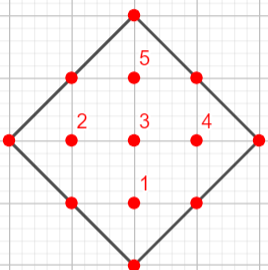
\includegraphics{img/points_on_omega_with_numbers.PNG}
    \caption{Discretized grid 2D}
    \label{fig:discretized grid 2D}
\end{figure}
\subsection{}
We have dirichlet boundary conditions. Because of that we will have a full rank $L_h$. Since we have regular points on the boundary we get the normal five point stencil. By using the ordering as seen in figure \eqref{fig:discretized grid 2D} with $u_h=\mtr{u_1&u_2&u_3&u_4&u_5}^T$ we get
\begin{align*}
    L_h = \frac{1}{h^2}\mtr{-4&0&1&0&0\\0&-4&1&0&0\\1&1&-4&1&1\\0&0&1&-4&0\\0&0&1&0&-4}
\end{align*}
With $u(x,y) = 1-\abs{x}$ for $(x,y)\in\partial\Omega$ we get the right hand side
\begin{align*}
    f_h = -\frac{1}{h^2}\mtr{
        2&
        1&
        0&
        1&
        2
    }^T.
\end{align*}
This comes from the fact that 
\newcommand{\abx}[1]{\abs{#1}}
\begin{align*}
    \frac{1}{h^2}\pth{1-\abs{0}} + \frac{1}{h^2}\pth{1-\abs{-0.5}} + \frac{1}{h^2}\pth{1-\abs{0.5}} + C
\end{align*}
where C is the terms within. So we see that when we move the known terms to the right hand side we get $-2/h^2$.
\subsection{Bonus mixed exercise: change of variables for finite differences}

\subsection{Bonus programming exercise: Lagrange multiplier}
Rewriting the problem with the given $u_*(x)$ we get
\begin{align*}
    -\nabla^2u(x) &= -6x\\
    \partial_\nu u(x) &= 2x \hspace{1em} x\in \squiggly{-1,1}
\end{align*}

\clearpage
\section*{Appendix}
\end{document}
